\chapter{Fazit}
\label{cha:Fazit}
Ich habe im letzten Jahr zunächst durch das Projekt und anschließend durch das Schreiben darüber einiges gelernt. Abgesehen von den technischen Details, lernte ich mich längere Zeit mit einem Thema zu beschäftigen und das Thema von verschiedenen Perspektiven (Messung, Auswertung, Darstellung) zu betrachten und bearbeiten. 
\begin{figure}[h]
  \centering
     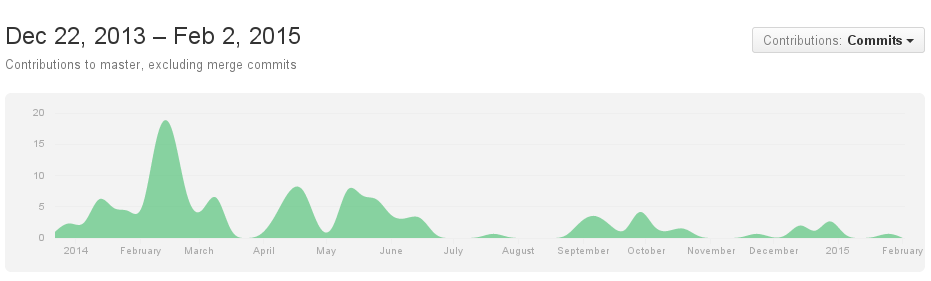
\includegraphics[width=\textwidth]{figures/Github_Umweltdatenmessung.png}
  \caption{Verlauf auf \gls{Github}}
  \label{fig:Github}
\end{figure}

Eine andere Erkenntnis aus dem Projekt ist, dass aus einer kleinen Idee ein ziemlich umfangreiches Projekt werden kann, welches sogar einen Preis gewinnt. (siehe Anhang \ref{anhang:präsentationen}) Angefangen hat alles am Beginn des Schuljahres 2013/14, als wir Ideen für ein \emph{Raspberry Pi}-Projekt recherchieren sollten. Ich hatte in den Ferien schon mit einem experimentiert und kam auf die Idee eine \emph{Wetterstation} zu bauen. Eine Woche später war das erste Programm fertig, welches Zufallszahlen, Prozessortemperatur und -auslastung mithilfe von Gnuplot als Diagramm anzeigt.\footnote{hier kann es noch gesehen werden: \href{https://gist.github.com/Findus23/d1187031f875b76a69e8}{gist.github.com/Findus23/d1187031f875b76a69e8} (\emph{csv2gnuplot.sh} ist nicht von mir)}

Durch das Schreiben dieser VWA und den Präsentationen (Anhang \ref{anhang:präsentationen}) 
habe ich gelernt technische Details so weit wie möglich allgemeinverständlich zu erklären und versuche bei den Präsentationen diese kurz zu fassen.

\section{Ausblick}
Wie es mit dem Projekt weitergehen wird, weiß ich noch nicht. Es gebe jedoch noch sehr viele Möglichkeiten zur Erweiterung. Vor allem können die Daten genutzt werden um andere Geräte zu steuern. So könnte der \emph{Raspberry Pi} zum Beispiel eine Heizung oder Beleuchtung ein- und ausschalten oder bei nicht optimaler Luftqualität im Klassenzimmer eine Warnung abgeben. 

Seit ich begonnen habe, sind einige neue Modelle des \emph{Raspberry Pi} herausgekommen, mit denen man mehr Sensoren hinzufügen könnte (zum Beispiel Helligkeit oder Lautstärke) oder die leistungsstärker sind und ohne zusätzliche Geräte eine grafische Darstellung auf einem Display anzeigen können.